\chapter{Single-Mode States of Light: Number, Coherent, Thermal, and Squeezed States}
\label{chap:e06}

\begin{chapteropening}
In the previous chapter we accomplished something big: we decomposed the entire electromagnetic field into a bunch of modes and proved that \emph{every mode is mathematically a harmonic oscillator}; so ``photon'' obtained a precise definition, as one excitation of some mode. But the same mode, like the same spring, can be in a myriad of quantum states. The question this chapter answers is plain, and also crucial: \textbf{within the same mode, exactly which kinds of shape can light take on? What do they look like differently?} We will find that whether the photon number is pinned down, whether the phase is stable, and whether the intensity fluctuates, make four typical states of light (number, coherent, thermal, and squeezed) leave utterly different ``click-statistics fingerprints'' even when their mean photon number is identical. To measure all four kinds of light with a single measurement, we first build one unified ruler: the \emph{zero-delay pair factor} \(b_2\). Then, for each kind of light, we compute its \(b_2\) by hand: the number state gives \(1-1/n\) (antibunching), the coherent state gives \(1\) (the Poisson baseline), the thermal state gives \(2\) (bunching). This ``extra factor of two'' is precisely the seed on which the later intensity interferometry (Hanbury Brown--Twiss) relies to work.
\end{chapteropening}

\section{A Unified Ruler: The Zero-Delay Pair Factor}
\label{sec:e06-b2}

First let us be clear about exactly what we want to measure. Chapter~\ref{chap:e05} already told us that behind every ``click'' of a telescope stands an annihilation operator \(\hat a\): some mode has one photon fewer. If we fix our gaze on the same mode and ask ``how strong is the tendency for two clicks to arrive almost simultaneously,'' this is one of the most essential distinctions between states of light; it shows up not in how bright the average is, but in \emph{whether photons like to cluster}.

Anyone can compute the mean photon number; it is just the expectation of the number operator \(\langle\hat n\rangle\). But looking only at the mean, the number, coherent, and thermal states can be completely identical (all tuned to \(\langle\hat n\rangle=\bar n\)), yet they are three utterly different kinds of light. What truly separates them is the matter of ``pairing'': within the same mode, how many pairs of photons can be assembled?

\paragraph{Why the factorial moment, not the square}
\label{sec:e06-why-factorial}

A beginner's most natural thought is to use \(\langle\hat n^2\rangle\) to measure ``pairing.'' This is exactly the first pitfall this section sets out to correct. Suppose the mode has \(N\) photons at this moment, and we want to count ``how many \emph{ordered photon pairs} can be picked from them.'' There are \(N\) ways to pick the first photon, and to pick the second, since it must be \emph{another} photon, not the one just picked, there are only \(N-1\) ways left. So the number of ordered pairs is
\[
  N\times(N-1)=N(N-1),
\]
not \(N\times N=N^2\). The term by which the two differ, \(N^2-N(N-1)=N\), is precisely the spurious term of ``pairing the same photon with itself.'' Physically, \textbf{the same photon cannot pair with itself}: once a detector absorbs it, it is gone, and it cannot possibly be absorbed simultaneously by a second detector. So for any quantity involving ``two clicks,'' the correct count must be \(N(N-1)\), the so-called \emph{second factorial moment}. This reasoning of ``self-pairing must be subtracted'' will be proved again at the operator level when we discuss the normal ordering of photodetection in Chapter~\ref{chap:e07}; here we first accept it from the combinatorial meaning of ``counting pairs.''

And so we define the zero-delay pair factor:
\begin{equation}
  b_2\equiv\frac{\langle\hat n(\hat n-1)\rangle}{\langle\hat n\rangle^{2}} .
  \label{eq:e06-b2def}
\end{equation}
\begin{formulaexplain}
The numerator \(\langle\hat n(\hat n-1)\rangle\) is ``on average how many pairs of photons can be assembled'' (with self-pairing subtracted); the denominator \(\langle\hat n\rangle^2\) is ``the baseline number of pairs there should be if photons were independent and arrived at random.'' \(b_2\) is the ratio of the two: by how many times the tendency of photons to cluster is amplified relative to the random baseline.
\end{formulaexplain}

Let us account for each symbol. \(\hat n=\hat a^\dagger\hat a\) is the number operator, with eigenvalues \(N=0,1,2,\dots\) being pure integers with no units; \(\langle\cdot\rangle\) is the expectation over the light state (an inner product for a pure state, a trace \(\operatorname{Tr}(\rho\,\cdot)\) for a mixed state). The numerator \(\langle\hat n(\hat n-1)\rangle\) is unitless, the ``mean number of pairs''; the denominator \(\langle\hat n\rangle^2\) is also unitless. So \(b_2\) is a pure number; it does not care how bright the mode is (the denominator has already normalized the brightness away), only about \emph{whether the tendency of photons to arrive in pairs within the same mode is more or less than the random baseline of ``each independent, not communicating with the others.''}

Why does the baseline given by ``independent randomness'' make the numerator exactly equal to the denominator? The next section will verify it rigorously when we compute the coherent state. Here we first set out the three criteria, the yardstick against which this chapter repeatedly checks:
\begin{itemize}
  \item \(b_2=1\): the \textbf{independent Poisson baseline}. Photons each come on their own, not communicating; seeing one does not change the probability of immediately seeing another.
  \item \(b_2>1\): \textbf{bunching}. Photons like to cluster, ``come together if at all,'' with a pairing probability above the random baseline; thermal light is exactly so.
  \item \(b_2<1\): \textbf{antibunching}, also called \emph{sub-Poisson}. Photons avoid each other, ``having come once, another is not easily coming right away,'' with a pairing probability below the random baseline; this is a purely quantum effect that classical waves cannot achieve.
\end{itemize}

With this ruler, we ``measure'' the four kinds of light one by one. The strategy is always the same: first write down the photon-number distribution \(P(N)\) of that state (or its density matrix), compute \(\langle\hat n\rangle\) and \(\langle\hat n(\hat n-1)\rangle\), and substitute into \eqref{eq:e06-b2def}. Every step is shown.

\section{Number States: Light with Photon Number Pinned Down}
\label{sec:e06-fock}

We begin with the most ``clean-cut'' light. Chapter~\ref{chap:e05} already met the number state \(|n\rangle\), also called the Fock state: it is an eigenstate of the number operator, \(\hat n|n\rangle=n|n\rangle\), meaning this mode has \emph{exactly} \(n\) photons, not one more, not one fewer, with no fluctuation whatsoever. Its counting distribution is a single, lone vertical line:
\begin{equation}
  P(N)=\delta_{Nn}=
  \begin{cases}
    1, & N=n,\\
    0, & N\neq n.
  \end{cases}
  \label{eq:e06-fock-dist}
\end{equation}
\begin{formulaexplain}
\(P(N)\) is the probability of ``counting \(N\) photons''; \(\delta_{Nn}\) is the Kronecker delta, equal to 1 only when \(N=n\) and 0 otherwise. It says that measuring the photon number of a number state always yields the same value \(n\), with no fluctuation at all.
\end{formulaexplain}

Precisely because \(P(N)\) is nonzero only at \(N=n\), all expectations degenerate into ``directly substitute \(N=n\).'' The mean photon number is
\[
  \langle\hat n\rangle=\sum_{N}N\,P(N)=n\cdot 1=n,
\]
and the second factorial moment likewise retains only the \(N=n\) term:
\[
  \langle\hat n(\hat n-1)\rangle=\sum_{N}N(N-1)\,P(N)=n(n-1).
\]
Substituting into the definition of the pair factor \eqref{eq:e06-b2def}:
\begin{equation}
  b_{2,\text{Fock}}=\frac{n(n-1)}{n^{2}}=\frac{n-1}{n}=1-\frac{1}{n}.
  \label{eq:e06-fock-b2}
\end{equation}
\begin{formulaexplain}
The pair factor of a number state differs from the random baseline \(1\) by exactly \(1/n\). The fewer the photons, the more pronounced the antibunching; when \(n=1\), \(b_2\) is pressed all the way down to \(0\).
\end{formulaexplain}

This result is worth chewing over. For any finite \(n\), \(b_2=1-1/n<1\): the number state is always \emph{antibunched}. The reason is plain to see: the mode has only \(n\) photons, and using one to count a pair leaves one less in ``stock,'' so the number of pairs that can be assembled \(n(n-1)\) is naturally fewer than the \(n^2\) of ``independent randomness.'' In particular, take the single-photon state \(n=1\):
\[
  b_{2,\text{Fock}}(n=1)=1-\frac{1}{1}=0.
\]
This is the \emph{ideal limit} of antibunching. The physical meaning is decisive: a mode has only one photon, and it is gone once absorbed, so it can never let two detectors each receive one \emph{simultaneously}; hence the ``pairing'' probability is exactly zero. This is the most precious quantum signature of a single-photon source, and resonance fluorescence in the laboratory can clearly produce \(b_2\to 0\) \citep{1977PhRvL..39..691K}.

A reminder, though: astronomical light almost never arrives in a pure number state. The countless independent emitters in the source region, the long propagation path, and the telescope and detector all mix unobserved degrees of freedom in, pulling \(b_2\) from \(0\) all the way back toward \(1\). The value of the number state here is to give us a \emph{lower-bound anchor} and a reminder: click statistics measure the correlations of photon number, not a continuous waveform. When \(n\to\infty\), \(b_2\to 1\) and the antibunching disappears; once photons are numerous, the quantum ``exclusivity'' is drowned in the numbers, foretelling why bright celestial objects rarely display non-classical statistics.

\section{Coherent States: The Light Most Like a Classical Laser}
\label{sec:e06-coherent}

At the end of Chapter~\ref{chap:e04} we previewed a quantum state ``closest to classical vibration''; now we formally bring it on. The coherent state \(|\alpha\rangle\) is defined as an eigenstate of the annihilation operator:
\begin{equation}
  \hat a\,|\alpha\rangle=\alpha\,|\alpha\rangle,
  \qquad
  \bar n\equiv\langle\hat n\rangle=|\alpha|^{2}.
  \label{eq:e06-coherent-def}
\end{equation}
\begin{formulaexplain}
\(|\alpha\rangle\) satisfies ``after being acted on by the annihilation operator it is unchanged, merely multiplied by a complex number \(\alpha\).'' \(\alpha\) is a dimensionless complex amplitude: its squared modulus \(|\alpha|^2\) gives the mean photon number \(\bar n\), its argument \(\arg\alpha\) gives the phase. This is the quantum version of a phase-stable, definite-amplitude ``classical wave.''
\end{formulaexplain}

First let us explain why this definition is ``classical.'' \(\alpha\) is a dimensionless complex number, and you may picture it as that ``rotating arrow'' (complex amplitude) of Chapter~\ref{chap:e01}: the modulus \(|\alpha|\) is the amplitude, the argument is the phase, both definite, with no phase jitter; this is exactly the picture of an ideal laser. A stable laboratory laser is, in many measurements, extremely close to a coherent state \citep{1963PhRv..131.2766G}. And that peculiar property ``\(\hat a|\alpha\rangle=\alpha|\alpha\rangle\)'' means: \emph{removing one photon from a coherent state, it is still the same coherent state}, like scooping one drop from a vast wave of consistent phase, the ripples do not change at all. This is what fundamentally distinguishes it from the number state.

\paragraph{Deriving the Poisson distribution from the definition}
\label{sec:e06-coherent-poisson}

Chapter~\ref{chap:e04} twice previewed that ``the photon number of a coherent state follows a Poisson distribution''; here we \emph{derive} it from the definition rather than parachuting it in. The only raw material is the eigenvalue equation \eqref{eq:e06-coherent-def}, plus the annihilation-operator action rule of Chapter~\ref{chap:e05}, \(\hat a|N\rangle=\sqrt{N}\,|N-1\rangle\).

\textbf{Step one: write the coherent state as a superposition of number states.} The number states \(\{|N\rangle\}\) are a complete basis of this mode, so any single-mode state can be expanded as a linear combination of them. Let
\[
  |\alpha\rangle=\sum_{N=0}^{\infty}c_N\,|N\rangle,
\]
where the undetermined coefficient \(c_N=\langle N|\alpha\rangle\) is the amplitude of ``the \(N\)-photon component in this state.'' Substitute it into the left side of the eigenvalue equation, using \(\hat a|N\rangle=\sqrt{N}\,|N-1\rangle\) (note the \(N=0\) term is annihilated and does not contribute):
\[
  \hat a\,|\alpha\rangle
  =\sum_{N=1}^{\infty}c_N\sqrt{N}\,|N-1\rangle
  =\sum_{M=0}^{\infty}c_{M+1}\sqrt{M+1}\,|M\rangle,
\]
where the last step relabels with \(M\equiv N-1\). And the right side of the eigenvalue equation is
\[
  \alpha\,|\alpha\rangle=\sum_{M=0}^{\infty}\alpha\,c_M\,|M\rangle.
\]
\textbf{Step two: match coefficients number state by number state, obtaining a recursion.} Both sides are expansions in the number-state basis, so corresponding coefficients must be equal; thus for each \(M\):
\[
  c_{M+1}\sqrt{M+1}=\alpha\,c_M
  \quad\Longrightarrow\quad
  c_{M+1}=\frac{\alpha}{\sqrt{M+1}}\,c_M .
\]
\textbf{Step three: solve the recursion.} Climbing up rung by rung from \(c_0\), each added photon multiplies by an \(\alpha/\sqrt{N}\):
\[
  c_1=\frac{\alpha}{\sqrt1}c_0,\quad
  c_2=\frac{\alpha}{\sqrt2}c_1=\frac{\alpha^2}{\sqrt{2!}}c_0,\quad\dots\quad
  c_N=\frac{\alpha^{\,N}}{\sqrt{N!}}\,c_0 .
\]
\textbf{Step four: normalization fixes \(c_0\).} Require \(\langle\alpha|\alpha\rangle=\sum_N|c_N|^2=1\). Substituting the above and calling by name the exponential series \(\sum_{N}x^N/N!=e^{x}\) (here \(x=|\alpha|^2\)):
\[
  \sum_{N=0}^{\infty}|c_N|^2
  =|c_0|^2\sum_{N=0}^{\infty}\frac{|\alpha|^{2N}}{N!}
  =|c_0|^2\,e^{|\alpha|^2}=1
  \quad\Longrightarrow\quad
  |c_0|^2=e^{-|\alpha|^2}.
\]
Take the positive real \(c_0=e^{-|\alpha|^2/2}\) (the phase is free to choose, not affecting the probability). At this point the number-state expansion of the coherent state is completely determined. \textbf{Step five: read off the photon-number probability.} The probability of counting \(N\) photons is precisely the squared modulus of that component amplitude:
\begin{equation}
  P(N)=\big|\langle N|\alpha\rangle\big|^2=|c_N|^2
  =\frac{|\alpha|^{2N}}{N!}\,e^{-|\alpha|^2}
  =e^{-\bar n}\,\frac{\bar n^{\,N}}{N!},
  \qquad N=0,1,2,\dots
  \label{eq:e06-poisson}
\end{equation}
\begin{formulaexplain}
\(P(N)\) is the probability of counting \(N\) photons; \(\bar n=|\alpha|^2\) is the mean photon number; \(N!\) is the normalization of discrete counting. It is derived all the way from the eigenvalue equation, and it is exactly the ``independent random arrival'' Poisson distribution of Chapter~\ref{chap:e03}; the photons of a coherent state are independent, each coming on its own.
\end{formulaexplain}

The last step used \(\bar n=|\alpha|^2\), converting the complex amplitude into the mean photon number. Equation \eqref{eq:e06-poisson} is the \textbf{Poisson distribution}, and it is not asserted but forced out step by step from ``\(\hat a|\alpha\rangle=\alpha|\alpha\rangle\)'': the eigenvalue equation gives the recursion, the recursion gives the coefficients, normalization fixes the constant, and the squared modulus gives the probability. Here \(\bar n=|\alpha|^2\) is unitless, and \(N!\) is the factorial of \(N\). Equation \eqref{eq:e06-poisson} is \emph{exactly of the same form} as the Poisson distribution in Chapter~\ref{chap:e03} when we discussed shot noise; this is no coincidence: the photons of a coherent state are mutually independent random events, precisely the source of shot noise, with variance equal to mean \(\operatorname{Var}(N)=\bar n\).

\paragraph{Computing the pair factor of a coherent state by hand}
\label{sec:e06-coherent-b2}

Now measure it with the ruler. To compute \(b_2\), we need the second factorial moment \(\langle N(N-1)\rangle\). Substituting the Poisson distribution \eqref{eq:e06-poisson} into the sum, without omitting a step:
\[
  \langle N(N-1)\rangle
  =\sum_{N=0}^{\infty}N(N-1)\,e^{-\bar n}\frac{\bar n^{\,N}}{N!}.
\]
\textbf{Step one: cut off the terms that vanish.} Each term of the sum carries the factor \(N(N-1)\). When \(N=0\), \(N(N-1)=0\); when \(N=1\), \(N(N-1)=1\cdot 0=0\). So the \(N=0\) and \(N=1\) terms make \emph{no contribution} to the sum, and we can start summing directly from \(N=2\):
\[
  \langle N(N-1)\rangle
  =\sum_{N=2}^{\infty}N(N-1)\,e^{-\bar n}\frac{\bar n^{\,N}}{N!}.
\]
\textbf{Step two: cancel the factorial.} Note the definition of the factorial \(N!=N(N-1)(N-2)!\), so \(N(N-1)/N!=1/(N-2)!\). This step cleanly eliminates the obstructive \(N(N-1)\):
\[
  \langle N(N-1)\rangle
  =e^{-\bar n}\sum_{N=2}^{\infty}\frac{\bar n^{\,N}}{(N-2)!}.
\]
\textbf{Step three: change variables in the sum.} Let \(m\equiv N-2\) (so \(N=2\) corresponds to \(m=0\), and \(N\to\infty\) corresponds to \(m\to\infty\)), and split \(\bar n^{\,N}=\bar n^{\,2}\cdot\bar n^{\,m}\), pulling the sum-independent \(\bar n^2\) outside:
\[
  \langle N(N-1)\rangle
  =e^{-\bar n}\,\bar n^{2}\sum_{m=0}^{\infty}\frac{\bar n^{\,m}}{m!}.
\]
\textbf{Step four: use the exponential series.} That last sum is exactly the Taylor series of the exponential function \(\sum_{m=0}^{\infty}\bar n^{\,m}/m!=e^{\bar n}\), a standard result we call by name. So \(e^{-\bar n}\) and \(e^{\bar n}\) cancel exactly:
\[
  \langle N(N-1)\rangle
  =e^{-\bar n}\,\bar n^{2}\,e^{\bar n}
  =\bar n^{2}.
\]
Clean and neat. Since \(\langle N\rangle=\bar n\), substituting into the definition of the pair factor \eqref{eq:e06-b2def}:
\begin{equation}
  b_{2,\text{coh}}=\frac{\langle N(N-1)\rangle}{\langle N\rangle^{2}}
  =\frac{\bar n^{2}}{\bar n^{2}}=1.
  \label{eq:e06-coherent-b2}
\end{equation}
\begin{formulaexplain}
The pair factor of a coherent state is exactly \(1\), independent of the brightness \(\bar n\). It is the \emph{independent Poisson baseline} on our yardstick: photons each come on their own, with a pairing probability neither more nor less.
\end{formulaexplain}

This \(b_2=1\) is the rigorous source of the ``independent random baseline'' in \eqref{eq:e06-b2def}. Physically it says something very plain: \textbf{seeing one photon in a coherent state does not change the conditional probability of immediately seeing another}. Photons neither communicate, nor pair up, nor avoid one another; they are purely independent. This also explains why a coherent state is neither bunched nor antibunched; it sits exactly on the dividing line between classical and quantum, the ``most classical quantum state.'' A stable laser is approximately so; but beware, \emph{a celestial narrow-line or high-brightness-temperature source is not automatically a coherent state}: independent emitting regions, turbulent velocity fields, and multiple scattering paths all smear the phase, and the result is instead closer to the thermal state of the next section.

\section{Thermal States: The Light of Stellar Continua}
\label{sec:e06-thermal}

Now for the light that astronomers most often deal with. The single-mode statistics of stellar continua, the scattered light of interplanetary dust, and the vast majority of incoherent sources all start from the thermal state. It has no fixed phase and is a \emph{mixed state} in the photon-number basis, with density matrix
\begin{equation}
  \rho_{\text{th}}=\sum_{N=0}^{\infty}
  \frac{\bar n^{\,N}}{(1+\bar n)^{\,N+1}}\,|N\rangle\langle N|,
  \label{eq:e06-thermal-rho}
\end{equation}
\begin{formulaexplain}
\(\rho_{\text{th}}\) is the thermal-state density matrix; it is an \emph{incoherent} mixture of the number states \(|N\rangle\), with weights decreasing geometrically; \(\bar n\) is the mean occupation of this mode. The thermal state has no phase information, only ``the probability of each photon number occurring.''
\end{formulaexplain}

First understand this expression. \(|N\rangle\langle N|\) is the operator projecting onto ``exactly \(N\) photons,'' and the coefficient in front is the probability of counting \(N\) photons
\[
  P(N)=\frac{\bar n^{\,N}}{(1+\bar n)^{\,N+1}}
  =\frac{1}{1+\bar n}\left(\frac{\bar n}{1+\bar n}\right)^{N}.
\]
This is a \textbf{geometric distribution}, that is, the Bose--Einstein distribution encountered when deriving the boson occupation in Chapter~\ref{chap:e05}: the probability decreases monotonically with \(N\), but drags a long tail of high photon number. It is precisely this tail that makes thermal light like to ``cluster'' more than coherent light. To verify normalization, use the geometric-series sum \(\sum_{N=0}^\infty q^N=1/(1-q)\) (here the common ratio \(q=\bar n/(1+\bar n)<1\), convergent), giving \(\sum_N P(N)=\frac{1}{1+\bar n}\cdot\frac{1}{1-q}=\frac{1}{1+\bar n}\cdot(1+\bar n)=1\), correct.

\paragraph{Computing the pair factor of a thermal state by hand}
\label{sec:e06-thermal-b2}

We want two things: the mean \(\langle N\rangle\) and the second factorial moment \(\langle N(N-1)\rangle\). Both start from the geometric distribution and are computed directly with the ready-made trick of ``differentiating the geometric series term by term'' from Chapter~\ref{chap:e05}, without borrowing any outside help; the variance \(\operatorname{Var}(N)\) is then read off as a by-product to explain the physics of bunching.

\textbf{The mean.} This step was already computed in Chapter~\ref{chap:e05} with the ``differentiate the geometric series term by term'' trick, the conclusion being
\[
  \langle N\rangle=\sum_{N=0}^{\infty}N\,P(N)=\bar n.
\]
That is, the parameter \(\bar n\) in \eqref{eq:e06-thermal-rho} lives up to its name and is exactly the mean photon number.

\textbf{The second factorial moment: computed directly by differentiating the geometric distribution term by term.} This is the core quantity of this section, and we do not borrow any unproven variance but compute it term by term from the geometric distribution \eqref{eq:e06-thermal-rho}, by the same method as the ``differentiate the geometric series'' used for the mean in Chapter~\ref{chap:e05}. For clean notation, write the common ratio
\[
  q\equiv\frac{\bar n}{1+\bar n}\in(0,1),
  \qquad\text{so that}\quad 1-q=\frac{1}{1+\bar n},\quad P(N)=(1-q)\,q^{N}.
\]
Everything starts from the most basic geometric series (convergent only for common ratio \(|q|<1\), satisfied here):
\[
  \sum_{N=0}^{\infty}q^{N}=\frac{1}{1-q}.
\]
Differentiating both sides once with respect to \(q\) gives that one formula used for the mean in Chapter~\ref{chap:e05}, \(\sum_N N q^{N-1}=1/(1-q)^2\); we here \emph{differentiate once more}, ``knocking'' the \(N(N-1)\) out of the power:
\[
  \frac{d^{2}}{dq^{2}}\sum_{N=0}^{\infty}q^{N}
  =\sum_{N=0}^{\infty}N(N-1)\,q^{\,N-2}
  =\frac{2}{(1-q)^{3}} .
\]
This step calls by name a standard result: \emph{for a convergent power series, term-by-term differentiation and summation can be interchanged} (for \(0<q<1\) the series converges uniformly in a neighborhood of \(q\), so it is legitimate). The right-hand side is obtained by differentiating \((1-q)^{-1}\) twice. Multiplying both sides by \(q^{2}\), restoring the power to \(q^{N}\):
\[
  \sum_{N=0}^{\infty}N(N-1)\,q^{N}=\frac{2q^{2}}{(1-q)^{3}} .
\]
Now equipping each term with the leading normalization factor \((1-q)\) gives the expectation we want:
\[
  \langle N(N-1)\rangle
  =(1-q)\sum_{N=0}^{\infty}N(N-1)\,q^{N}
  =(1-q)\cdot\frac{2q^{2}}{(1-q)^{3}}
  =\frac{2q^{2}}{(1-q)^{2}}
  =2\left(\frac{q}{1-q}\right)^{2}.
\]
Finally convert \(q\) back to \(\bar n\): from \(q=\bar n/(1+\bar n)\) and \(1-q=1/(1+\bar n)\) we get \(q/(1-q)=\bar n\), so
\begin{equation}
  \langle N(N-1)\rangle=2\bar n^{2}.
  \label{eq:e06-thermal-fm}
\end{equation}
\begin{formulaexplain}
The second factorial moment of a thermal state is \(2\bar n^2\), exactly \emph{twice} the \(\bar n^2\) of a coherent state. This extra factor of two is the entire source of the later \(b_2=2\) (bunching); it is computed by hand by differentiating the geometric distribution term by term, without invoking any unproven fact.
\end{formulaexplain}

\textbf{Read off the variance in passing, to make bunching clear.} Since the factorial moment is now in hand, the variance is its direct by-product: using \(\langle N^2\rangle=\langle N(N-1)\rangle+\langle N\rangle\),
\begin{equation}
  \operatorname{Var}(N)=\langle N^{2}\rangle-\langle N\rangle^{2}
  =\big[2\bar n^{2}+\bar n\big]-\bar n^{2}
  =\bar n+\bar n^{2}=\bar n(1+\bar n).
  \label{eq:e06-thermal-var}
\end{equation}
\begin{formulaexplain}
The variance of a thermal state exceeds the Poisson \(\bar n\) by one term \(\bar n^2\). The first term \(\bar n\) is the unavoidable shot noise (``photons come one at a time''), and the second term \(\bar n^2\) is the \emph{intensity fluctuation} peculiar to thermal light, precisely what brings bunching.
\end{formulaexplain}

Read the variance \eqref{eq:e06-thermal-var} split into two parts: \(\operatorname{Var}(N)=\underbrace{\bar n}_{\text{shot noise}}+\underbrace{\bar n^{2}}_{\text{intensity fluctuation}}\). The first term \(\bar n\), as in the coherent state, is the unavoidable shot noise from ``photons being discrete''; the second term \(\bar n^2\) is the \emph{extra} that the thermal state carries, coming from the intensity of the light field itself fluctuating randomly: thermal light is sometimes bright, sometimes dim, and when bright the photons all become more numerous together, when dim they all become fewer together. This ``excess variance'' is the root of bunching; please remember it. With the factorial moment \eqref{eq:e06-thermal-fm}, substitute directly into the definition of the pair factor \eqref{eq:e06-b2def}:
\begin{equation}
  b_{2,\text{th}}=\frac{\langle N(N-1)\rangle}{\langle N\rangle^{2}}
  =\frac{2\bar n^{2}}{\bar n^{2}}=2.
  \label{eq:e06-thermal-b2}
\end{equation}
\begin{formulaexplain}
The pair factor of a thermal state is exactly \(2\), independent of brightness. It is \emph{twice} the random baseline: the probability of thermal-light photons arriving in pairs is twice that of the independent random case. This is bunching.
\end{formulaexplain}

This \(b_2=2\) is the centerpiece of this chapter. Where does that ``extra factor'' (the \(1\) by which \(2\) exceeds the baseline \(1\)) come from? It is \emph{not} a detector effect, nor some new particle interaction, but the direct consequence of that second intensity-fluctuation term \(\bar n^2\) above: when thermal light has excess intensity in some short coherence time, multiple photons \emph{together} more easily arrive; when intensity is low, they \emph{together} become fewer. This ``all more together, or all fewer together'' advance-and-retreat in unison makes photons tend to arrive in pairs and in groups; this is the microscopic picture of bunching.

The importance of this cannot be overstated: \textbf{the \(b_2=2\) of thermal light is precisely the seed on which Hanbury Brown--Twiss (intensity interferometry) relies to work}. In the 1950s Hanbury Brown and Twiss, by measuring exactly this excess correlation of photon arrival on two detectors, first measured stellar angular diameters without amplitude interferometry \citep{1956Natur.177...27B,1957RSPSA.242..300B}. Without that extra factor of thermal light, there would be no measurable correlation peak. In Chapter~\ref{chap:e08} we will translate this \(b_2=2\) precisely into the second-order coherence function \(g^{(2)}(0)=2\), and in Chapter~\ref{chap:e10} turn it into a tool for measuring angular diameters.

One necessary reminder: the \(\bar n\) here is the \emph{single-mode} mean occupation, not the total photon rate the telescope receives per second. Moreover, a real observation is always a sum of many modes (the \(M\) of Chapter~\ref{chap:e05}), and the multi-mode average dilutes this ``excess variance,'' making the measured bunching contrast smaller than the single-mode ideal of \(2\). This dilution effect is also a core matter to be handled repeatedly in Chapters~\ref{chap:e08} and \ref{chap:e10}.

Figure~\ref{fig:e06-count-distributions} draws the counting distributions of the three kinds of light at the same mean photon number together, and the source of the difference is seen at a glance.

\begin{figure}[tbp]
\centering
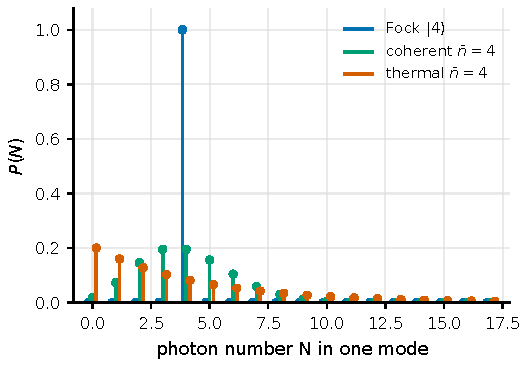
\includegraphics[width=0.82\linewidth]{figures/generated/chapter_03/ch03_state_count_distributions.pdf}
\caption{Near the same mean photon number, the number, coherent, and thermal states give completely different counting distributions \(P(N)\). The number state is a single pinned-down vertical line (no fluctuation in photon number, \(b_2=1-1/n<1\)); the coherent state is a Poisson distribution, with width about \(\sqrt{\bar n}\) (\(b_2=1\)); the thermal state is a geometric distribution, dragging a long tail of high photon number (\(b_2=2\), bunching). It is precisely this tail that makes thermal light more likely to arrive ``in pairs'' at zero delay.}
\label{fig:e06-count-distributions}
\end{figure}

The lesson of Figure~\ref{fig:e06-count-distributions} is extremely simple: \emph{the mean photon number is not everything}. The number state has no photon-number fluctuation, the coherent state has Poisson fluctuation, and the thermal state additionally bears a layer of intensity fluctuation. What astronomical intensity interferometry exploits is precisely this last layer of fluctuation of the thermal state.

\section{Squeezed States: Relocating the Quantum Noise}
\label{sec:e06-squeezed}

The first three kinds of light concerned ``how the photon number is distributed.'' The squeezed state is about something different: \emph{quantum noise can be redistributed between two orthogonal field components}. It does not change the language of photon-pairing statistics but returns to the quadrature picture of Chapter~\ref{chap:e04}.

First define a quadrature operator at a phase angle \(\theta\):
\begin{equation}
  \hat X_\theta=\frac{1}{2}\left(\hat a\,e^{-i\theta}+\hat a^{\dagger}e^{i\theta}\right).
  \label{eq:e06-quadrature}
\end{equation}
\begin{formulaexplain}
\(\hat X_\theta\) is the ``projection'' of the field along the phase direction \(\theta\), a generalization of the position/momentum operators of Chapter~\ref{chap:e04}: \(\theta=0\) gives the ``position''-like component, \(\theta=\pi/2\) gives the ``momentum''-like component. It is dimensionless and measures the coordinate of the field along some direction in phase space.
\end{formulaexplain}

Let us account for each. \(\hat X_\theta\) is dimensionless; \(\theta\) is the phase-space ``viewing angle'' we choose (in radians); \(\hat a,\hat a^\dagger\) are old acquaintances. Taking \(\theta=0\) gives \(\hat X_0=\tfrac12(\hat a+\hat a^\dagger)\), proportional to the position operator \(\hat x\) of Chapter~\ref{chap:e04}; taking \(\theta=\pi/2\) gives \(\hat X_{\pi/2}=\tfrac{1}{2i}(\hat a-\hat a^\dagger)\), proportional to the momentum operator \(\hat p\). These two orthogonal directions are the ``horizontal and vertical axes'' of phase space.

The key quantum fact is: \textbf{the vacuum state (and any coherent state) has equal fluctuation in every direction}, with variance \(1/4\) in all. This baseline value is not hard to compute, and it is worth cashing out on the spot: it uses only two properties of the vacuum, \(\hat a|0\rangle=0\) and the commutation relation \([\hat a,\hat a^\dagger]=1\). In the vacuum \(\langle\hat X_\theta\rangle=0\) (the expectations of both \(\hat a,\hat a^\dagger\) are zero), so the variance equals \(\langle\hat X_\theta^2\rangle\). Expanding the square of the definition \eqref{eq:e06-quadrature}:
\[
  \hat X_\theta^{2}
  =\frac14\big(\hat a\,e^{-i\theta}+\hat a^\dagger e^{i\theta}\big)^2
  =\frac14\big(\hat a^2 e^{-2i\theta}+\hat a^{\dagger 2}e^{2i\theta}
     +\hat a\hat a^\dagger+\hat a^\dagger\hat a\big).
\]
Take the vacuum expectation term by term: the term with \(\hat a^2\) vanishes because \(\hat a|0\rangle=0\); the term with \(\hat a^{\dagger2}\), its Hermitian conjugate, likewise vanishes; \(\hat a^\dagger\hat a\,|0\rangle=0\) (the number operator acting on the vacuum is zero); only \(\langle 0|\hat a\hat a^\dagger|0\rangle\) remains, and using \(\hat a\hat a^\dagger=\hat a^\dagger\hat a+[\hat a,\hat a^\dagger]=\hat n+1\) gives \(\langle0|\hat a\hat a^\dagger|0\rangle=0+1=1\). So
\[
  \Delta X_\theta^{2}\big|_{\text{vacuum}}=\langle\hat X_\theta^2\rangle
  =\frac14\cdot 1=\frac{1}{4}\qquad(\text{for all }\theta).
\]
The result is independent of \(\theta\), showing precisely that the vacuum is an isotropic ``circular blob'' in phase space; this is also the starting point of the next section's phase-space picture. The Heisenberg uncertainty requires the product of the variances of two orthogonal directions to be no less than \(\tfrac{1}{16}\), and the vacuum saturates this minimum exactly (\(\tfrac14\times\tfrac14=\tfrac1{16}\)).

What the squeezed state does is \emph{squash} this circular blob: pressing the variance along some direction below \(1/4\), at the cost of the variance of the conjugate direction being correspondingly raised. Let the squeezing parameter be \(r\ge0\); then
\begin{equation}
  \Delta X_{\text{sq}}^{2}=\frac{1}{4}\,e^{-2r},
  \qquad
  \Delta X_{\text{anti}}^{2}=\frac{1}{4}\,e^{+2r}.
  \label{eq:e06-squeeze-var}
\end{equation}
\begin{formulaexplain}
The variance of the squeezed direction is multiplied by \(e^{-2r}<1\) (noise decreases), and the variance of the anti-squeezed direction is multiplied by \(e^{+2r}>1\) (noise increases). The larger \(r\), the ``flatter'' one direction and the ``fatter'' the other.
\end{formulaexplain}

This \(e^{\mp 2r}\) shape comes from the single-mode squeezing transformation: it multiplies the amplitude scale of phase space along one quadrature direction by \(e^{-r}\), so the variance (the square of the scale) is multiplied by \(e^{-2r}\); the scale of the conjugate direction is multiplied by \(e^{+r}\), the variance by \(e^{+2r}\). Most crucial is multiplying the two variances together:
\[
  \Delta X_{\text{sq}}^{2}\cdot\Delta X_{\text{anti}}^{2}
  =\frac14 e^{-2r}\cdot\frac14 e^{+2r}
  =\frac{1}{16}\,e^{-2r+2r}
  =\frac{1}{16}.
\]
The product is \emph{still} \(1/16\), exactly the same as the vacuum! This sentence is the key to understanding squeezing: \textbf{squeezing has not eliminated the quantum noise; it has merely moved the noise from one direction to another}: press down the gourd and the ladle pops up, the total conserved. You may make some quadrature component quieter than the vacuum, but you must let its conjugate component grow noisy to compensate.

The experimental literature often uses decibels (dB) to note the noise ratio relative to vacuum: \(10\log_{10}(e^{-2r})\). For example, a noise variance reduced to one tenth of the vacuum is \(-10\,\text{dB}\). Modern squeezed-light experiments near \(1064\,\text{nm}\) can already stably produce \(10\)--\(15\,\text{dB}\) of noise reduction, and it has been used in gravitational-wave detectors to press shot noise below the standard quantum limit \citep{1983Natur.306..141W,2016PhRvL.117k0801V}.

But a cold splash of water for astronomy: \textbf{ordinary stellar continua do not carry squeezing by default}. Thermal and coherent states have fluctuations no smaller than vacuum in every quadrature direction; there is no ``squashing'' to speak of. Squeezing is a non-classical state that must be carefully prepared with nonlinear optical processes (such as parametric down-conversion), and natural thermal sources like stars and nebulae do not produce it spontaneously. We introduce the squeezed state, first, to complete the full atlas of ``which kinds of light the same mode can hold,'' and second, because it is crucial on the \emph{instrument side}: future quantum-enhanced telescope back ends may use squeezed light to break through shot noise. But treating it as the default model of astronomical light is a misconception to avoid.

\section{The Weak Thermal Light Limit: A Line Laid Down for Super-Resolution}
\label{sec:e06-weak}

The last section pushes the thermal state into the most common corner of astronomy: \emph{every mode is actually quite dim}. Chapter~\ref{chap:e05} computed that in the visible the single-mode occupation of a star is \(\bar n_\nu\sim10^{-2}\ll1\). In this weak thermal light limit, the thermal state degenerates into a particularly simple, particularly useful form.

Starting from the geometric distribution, expand \(P(N)\) to lowest order when \(\bar n\ll 1\). The probability of zero photons is
\[
  P(0)=\frac{1}{1+\bar n}\simeq 1-\bar n+\mathcal O(\bar n^{2}),
\]
where we used the geometric-series expansion \((1+\bar n)^{-1}=1-\bar n+\bar n^2-\cdots\) (convergent for \(\bar n<1\)), keeping only to first order. The probability of one photon is
\[
  P(1)=\frac{\bar n}{(1+\bar n)^{2}}
  \simeq\bar n\,(1-2\bar n+\cdots)
  \simeq\bar n+\mathcal O(\bar n^{2}).
\]
The probability of two or more photons is
\[
  P(N\ge 2)=\mathcal O(\bar n^{2}),
\]
because \(P(2)=\bar n^2/(1+\bar n)^3\sim\bar n^2\), a higher-order small quantity. That is, in weak thermal light \emph{the vast majority of coherence-time windows are empty}, occasionally one window has one photon popping out, while two photons in the same window is a second-order rare event.

Writing this hierarchy as a density matrix gives the standard bookkeeping form of weak thermal light:
\begin{equation}
  \rho\simeq(1-\varepsilon)\,\rho_0+\varepsilon\,\rho_1+\mathcal O(\varepsilon^{2}),
  \qquad
  \varepsilon\equiv\bar n\ll 1,
  \label{eq:e06-weak}
\end{equation}
\begin{formulaexplain}
\(\rho_0=|0\rangle\langle 0|\) is the vacuum part (fraction \(1-\varepsilon\)), \(\rho_1=|1\rangle\langle 1|\) is the one-photon part (fraction \(\varepsilon\)), and \(\varepsilon=\bar n\) is the single-mode mean photon number. Weak thermal light is a sparse photon stream that is ``mostly empty, occasionally one.''
\end{formulaexplain}

Let us account for each: \(\rho_0\) is the density matrix of the vacuum state, \(\rho_1\) is the density matrix of the single-photon state, and the small parameter \(\varepsilon=\bar n\) is dimensionless, exactly equal to the lowest-order \(P(1)\) above, so \emph{it is exact to identify \(\varepsilon\) as ``the mean photon number of that mode in that time window.''} Equation \eqref{eq:e06-weak} says: the light state is almost entirely vacuum, with just a tiny bit of single-photon component mixed in. This ``tiny bit'' is precisely what carries the celestial information.

Why devote a whole section to it? Because it is the starting point of the later \textbf{quantum super-resolution}. Since a coherence-time window usually contains no photon and only occasionally one, what truly carries the spatial information of the celestial object is the spatial structure of that \emph{one-photon mode} that was detected. The weak-thermal-light super-resolution theory of Tsang, Nair, and Lu starts precisely from an expansion like \eqref{eq:e06-weak}, proving that as long as one can cleverly measure the mode of this single photon (rather than simply counting the intensity), one can break through the classical Rayleigh limit \citep{2015Optic...2..646T,2016PhRvX...6c1033T}. We will pick up this line in Chapter~\ref{chap:e12}, discussing how SPADE (spatial-mode demultiplexing) approaches the resolution limit of two stars extremely close together. This also fits naturally with the astronomical event table: the time windows of zero photons are never stored in the file at all; what remains in the data are those sparse single-photon clicks with time stamps.

\section{The Phase-Space Picture: Drawing the Four Kinds of Light on One Diagram}
\label{sec:e06-phasespace}

Let us gather this chapter onto one \emph{visible} diagram. Phase space uses two quadrature components \(X\) (horizontal axis) and \(P\) (vertical axis) to span a plane, drawing the quantum state of a mode as a ``probability cloud'' on this plane: the center of the cloud is the mean field, the fatness of the cloud is the fluctuation. As said in the previous section, the vacuum and coherent states have fluctuations of \(1/4\) in every direction, so they draw as an isotropic \emph{circular blob}. The four kinds of light each have their own look on this diagram:

\begin{itemize}
  \item \textbf{Vacuum state}: a circular blob at the origin, its radius set by the \(1/4\) fluctuation. This is the ``base'' of all noise.
  \item \textbf{Coherent state}: a circular blob \emph{of exactly the same size}, only translated to a distance \(|\alpha|\) from the origin. It moves the vacuum's circular blob as a whole, shape unchanged; so the coherent state is a ``displaced vacuum,'' with noise as small and as isotropic as the vacuum. This corresponds to its \(b_2=1\).
  \item \textbf{Thermal state}: a \emph{fatter circle still centered at the origin}. It has no fixed phase (the argument is completely random) and has intensity fluctuation, so the probability cloud spreads out in all directions, its radius growing with \(\bar n\). This ``fatter'' is precisely the phase-space image of the thermal state's extra variance \(\bar n^2\), also corresponding to its \(b_2=2\).
  \item \textbf{Squeezed state}: a \emph{squashed ellipse}. Along the squeezed direction it is narrow, below vacuum (\(\tfrac14 e^{-2r}\)), and along the conjugate direction it is propped fat (\(\tfrac14 e^{+2r}\)), but the area of the ellipse (the variance product \(1/16\) corresponding to the product of the two semi-axes) is the same as the circular blob: ``noise relocated, area conserved'' appears on the diagram as ``circle squashed into an equal-area ellipse.''
\end{itemize}

Figure~\ref{fig:e06-phase-space} draws these three ``clouds'' of the coherent, thermal, and squeezed states side by side.

\begin{figure}[tbp]
\centering
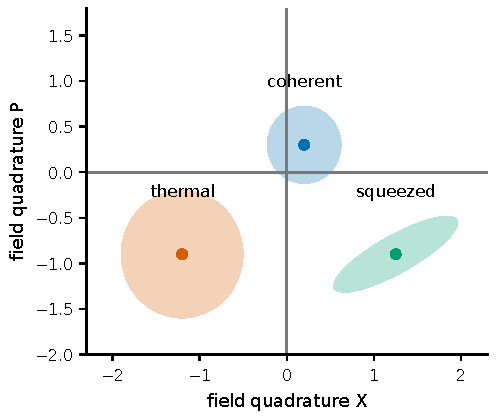
\includegraphics[width=0.72\linewidth]{figures/generated/chapter_03/ch03_phase_space_states.pdf}
\caption{The fluctuation shapes of three kinds of single-mode light state in phase space. The coherent state is a circular blob the same size as the vacuum, only translated (a ``displaced vacuum''); the thermal state, due to random phase and intensity fluctuation, spreads into a fatter circle; the squeezed state presses the fluctuation of one quadrature direction below vacuum while raising the conjugate direction, becoming an equal-area ellipse. Remember: what distinguishes different states of light is, first of all, the \emph{shape} of the fluctuations and correlations, not just the mean intensity.}
\label{fig:e06-phase-space}
\end{figure}

This phase-space diagram gives one take-away sentence: \emph{the distinction between different states of light shows up, first of all, as the shape of the fluctuations and correlations, not just the mean intensity}. The same brightness can be a well-behaved circular blob (coherent state), a restless fat circle (thermal state), or a squashed ellipse (squeezed state), and it is precisely these shapes that determine the pairing statistics of clicks on the detector. Carrying this diagram, we can enter Chapter~\ref{chap:e07} and see how these states of light truly become a string of analyzable events on a photodetector.

\section{Chapter Summary}
\label{sec:e06-summary}

\begin{itemize}
  \item \textbf{The ruler: the zero-delay pair factor} \(b_2=\langle\hat n(\hat n-1)\rangle/\langle\hat n\rangle^2\). The numerator uses the factorial moment \(\hat n(\hat n-1)\) rather than \(\hat n^2\), because ``the same photon cannot pair with itself'' and self-pairing must be subtracted. \(b_2=1\) is the independent Poisson baseline, \(>1\) bunching, \(<1\) antibunching (non-classical).
  \item \textbf{Number state \(|n\rangle\)}: \(P(N)=\delta_{Nn}\), photon number pinned down. \(\langle\hat n\rangle=n\), \(\langle\hat n(\hat n-1)\rangle=n(n-1)\), giving \(b_2=1-1/n<1\). The single photon \(n=1\) gives \(b_2=0\), the ideal limit of antibunching.
  \item \textbf{Coherent state \(|\alpha\rangle\)}: \(\hat a|\alpha\rangle=\alpha|\alpha\rangle\), \(\bar n=|\alpha|^2\), counting is Poisson. Term-by-term summation (cut off zero terms, cancel the factorial, change variables, use the exponential series) gives \(\langle N(N-1)\rangle=\bar n^2\), so \(b_2=1\). Seeing one photon does not change the probability of immediately seeing another.
  \item \textbf{Thermal state \(\rho_{\text{th}}\)}: geometric/Bose distribution, \(\langle N\rangle=\bar n\), \(\operatorname{Var}=\bar n(1+\bar n)\), \(\langle N(N-1)\rangle=2\bar n^2\), so \(b_2=2\). The extra factor comes from intensity fluctuation (more together when bright, fewer together when dim), precisely the seed of Hanbury Brown--Twiss bunching.
  \item \textbf{Squeezed state}: quadrature \(\hat X_\theta=\tfrac12(\hat a e^{-i\theta}+\hat a^\dagger e^{i\theta})\), vacuum variance \(1/4\); squeezed/anti-squeezed variance \(\tfrac14 e^{\mp 2r}\), the product still \(1/16\): the noise is relocated, not eliminated. Ordinary stellar light does not carry squeezing by default; it is mainly useful on the instrument side.
  \item \textbf{Weak thermal light limit}: for \(\bar n\ll1\), \(\rho\approx(1-\varepsilon)\rho_0+\varepsilon\rho_1\), \(\varepsilon=\bar n\), obtained from the lowest-order geometric distribution \(P(0)\approx1-\bar n\), \(P(1)\approx\bar n\). Most time windows are empty, and what carries the spatial information is that detected single-photon mode, leading to the super-resolution of Chapter~\ref{chap:e12}.
  \item \textbf{Phase space}: coherent state = displaced vacuum circular blob, thermal state = fatter circle, squeezed state = equal-area flat ellipse. What distinguishes states of light is, first of all, the shape of the fluctuations, not the mean intensity.
\end{itemize}

\medskip
\noindent\textbf{Questions to Ponder.}
\begin{enumerate}
  \item If you incoherently superpose two independent single-mode thermal beams (each with \(b_2=2\)) into one ``two-mode'' channel, will the observed pair factor be greater than 2, equal to 2, or less than 2? Is this consistent with the ``multi-mode dilution'' statement of Chapter~\ref{chap:e05}?
  \item For the same mean photon number \(\bar n=10\), what are the counting variances of the number, coherent, and thermal states? Which is the ``quietest'' and which the ``noisiest''?
  \item If some celestial source is measured to have \(b_2<1\), can you immediately assert it is a non-classical source? Before drawing the conclusion, which instrumental and mixing effects that could raise or lower \(b_2\) must you still rule out (recall the mode count \(M\) of Chapter~\ref{chap:e05})?
\end{enumerate}
